\newpage
\hypertarget{conBran tex}{}
\subsection{Branching with statement nodes}
\texHeader

\begin{itemize}

\item[$\blacktriangleright$] Before doing anything else, let's declare the method that will insert two new partitions into \texttt{box} when the
pattern in \texttt{grow} fails. Open \texttt{Box.eclass} and add the following signature: \syntax{initializeBox() : EBoolean}

\vspace{0.5cm}

\item[$\blacktriangleright$] Now modify \texttt{Box.grow()} by adding a nested \emph{if/else} construct, with \texttt{[addNewPartitionBox]} as the
first conditional, and a \emph{statement node} to invoke \texttt{initializeBox} if it fails. \emph{Statement nodes}\index{Statement Nodes} are specified via:
\syntax{`<' method\_call `>'\\
}
% \\
% With:\\}


\texttt{grow} should now resemble Fig.~\ref{eclipse:updateGrow}.

\vspace{0.5cm}

\begin{figure}[htp]
\begin{center}
  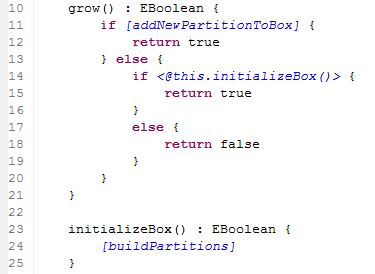
\includegraphics[width=0.5\textwidth]{eclipse_updateGrow}
  \caption{Extending \texttt{grow} with a \emph{statement node}}
  \label{eclipse:updateGrow}
\end{center}
\end{figure}

\vspace{0.5cm}

\item[$\blacktriangleright$] Next we have to specify our newest method. Create a new pattern called \texttt{buildPartitions} in its scope. Complete
the pattern as illustrated in Fig.~\ref{eclipse:pattBuildParts}.

\item[$\blacktriangleright$] As you can see, we have created a NAC that can only be fulfilled if the box has absolutely no partitions at all. This means that if
a box is completely empty, it will be initialized for the first time with two partitions (according to \texttt{buildPartitions}), and is guaranteed to remain in
a valid state via \texttt{grow}.

\clearpage

\vspace*{2cm}

\begin{figure}[htp]
\begin{center}
  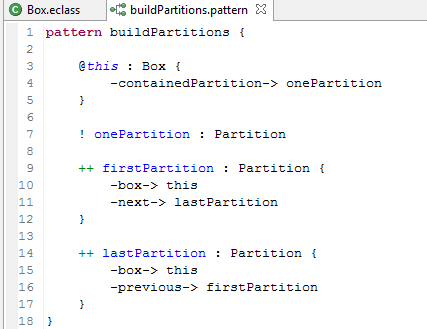
\includegraphics[width=0.7\textwidth]{eclipse_buildPartitionsPattern}
  \caption{NAC initalizing an empty box}
  \label{eclipse:pattBuildParts}
\end{center}
\end{figure}

\item[$\blacktriangleright$] That's it! Save and build your metamodel to make sure no errors exist. To see how this is depicted in the visual syntax, check out
Fig.~\ref{ea:newGrowControl} and Fig.~\ref{ea:buildPartitions}.

\end{itemize}
